%!TEX root = ../master_thesis.tex
\chapter{Introduction}
\label{ch:introduction}
In past two decades, deep learning (DL) research has gained a lot of popularity and has been widely used to solve various problems in artificial intelligence (AI) like object recognition in computer vision, sentiment classification in natural language processing (NLP), etc. The majority of success in DL research is in the discriminative class of models, where a classifier is trained to map the input data to its label class. The label class can be a discrete number for classification or a continuous value for regression.
A particular class of emerging deep learning research focuses on generative models (GMs) where the objective is to estimate the joint probability distribution of the input data and class labels. In recent years GMs have attracted a lot of interest mainly due to advancement in deep learning methods and computational resources. \citet{goodfellow2014generative} proposed generative adversarial networks (GANs) which efficiently learn to generate samples from high dimensional probability distributions in an adversarial setting. GANs have achieved state-of-the-art performance for various computer vision tasks. For instance, generating high-resolution images (\cite{karras2017progressive}) and multi-stage generation (\cite{denton2015deep}, \cite{karras2017progressive}). However, their application for audio or speech data is still limited. 
%One downside of GANs is that the training instabilities are encountered in form of mode collapse or oscillatory loss behavior. We will discuss it in Section~\ref{subsec:ch_gan_train}.
%Over the past few years, various improvements have been proposed for GAN training (e.g.~\cite{karras2017progressive},~\cite{arjovsky2017wasserstein},~\cite{petzka2017regularization}).

A problem often encountered in developing ML systems is the limited amount of data at the training time. This results in low performance when evaluated on samples different from those in the training set. The low diversity of samples at training time could also lead to poor generalization performance.
%The poor generalization can be attributed to low diversity of samples in the training data. Thus, for a model to generalize well one of the requirement is that the training samples should reflect the true population in terms of data distribution. 
Thus, for a robust model, one of the requirement is that the training samples should reflect the true population of samples in the data distribution. For example, to detect an image of a cat we need to show the model images of different kinds of cats during training. This allows the model to generalize the notion of a cat. An interesting application of GANs is to use them for generating high-fidelity data which then can be used to augment the training of ML systems. 

GANs learn to generate data by applying a parametric transformation on a noise distribution. One limitation in this setup is of generating data with some predefined attributes. For example, generating an image of a car given we define the shape of a car.
%A common problem encountered in this approach is of sampling from an appropriate noise distribution to generate images of required class. 
An interesting class of GANs (\cite{zhu2017unpaired},~\cite{liu2017unsupervised}) addresses this issue by posing it as a translation problem from data of one domain to that of another domain. The main idea in this setup is to learn specific characteristics or features of an image in the source domain and then use them to generate an image in the target domain. In previous example, shape of the car can be one domain and image as the other domain. Figure~\ref{fig:imagetoimage} further gives an example of translating images from a given source domain to the desired target domain.

\begin{figure}
    \centering
    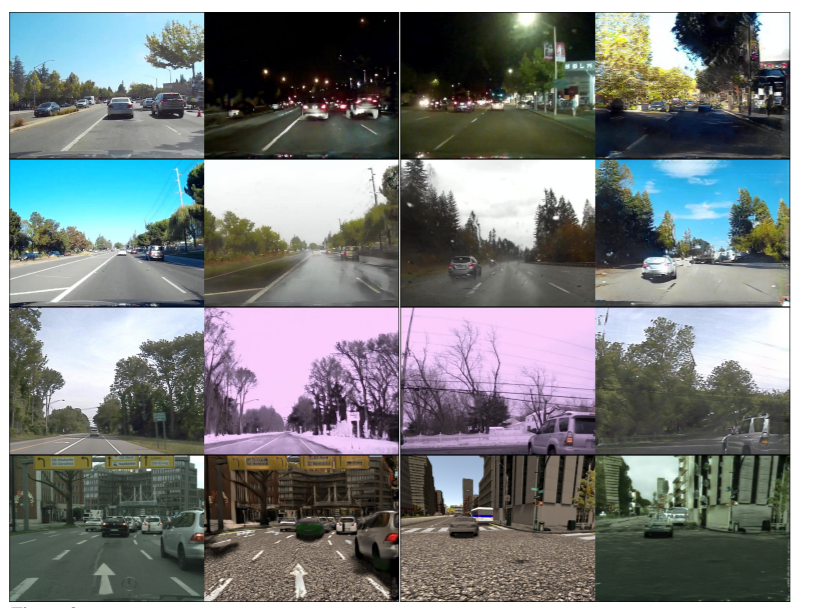
\includegraphics[width=0.85\columnwidth]{master_thesis_template/figs/image-to-image.PNG}
    \caption[An example of image to image translation.]{An example of image to image translation. Rows from top to bottom are tasks: day to night, sunny to rainy, summer to snowy, winter to summer and vice versa. The first and third column from the left are examples of input domain and second and fourth are example of translated images. Taken from \cite{liu2017unsupervised}}
    \label{fig:imagetoimage}
\end{figure}


DL models have already offered a significant promise in building robust speech detection systems. However, such systems are usually limited and perform poorly when evaluated on unseen data. For example, consider speech assistant systems which are trained on the task of transcribing speech to text.
%Such systems often fail when evaluated on the out of distribution speakers. 
Evaluation of such systems on an unseen set of speakers often fails. This is mainly due to the limited diversity of speakers in the training data. A robust system should learn the high variability of the features like phonetics of a speaker, accent and dialect associated with a language, etc. This requirement is often difficult to fulfill due to constraints imposed by the data collection process. Thus, an unsupervised framework to generate speech of the target domain is of great help for the development of robust systems. Furthermore, the existence of such a system can be used for voice privacy in online gaming platforms. The players can choose to be anonymous by translating their voice to an arbitrary choice of voice. 

In this thesis, following the work of \citet{liu2017unsupervised}, we propose a GAN framework for unsupervised speech-to-speech synthesis. In our work, we define speech-to-speech synthesis as the task of translating the voice of male speakers to female speakers and vice versa. Since our framework is completely unsupervised it requires no pairing of samples of male and female speakers for training.
%The robustness of such a system depends on the diversity of speech signals present at the time of training.

Speech signals are slow time-varying signals represented as a waveform of time-amplitude variations. \citet{oord2016wavenet} proposed an autoregressive model to generate high-quality speech signals from the time domain representation. However, the approach is limited and results in a slow real-time inference. This is mainly attributed to the high sampling rate of speech data which makes it computationally difficult to generate speech waveform in real-time. An alternative to the time-amplitude representation is the time-frequency representation where a signal is expressed in terms of the energy of its frequency components. Recently, several GAN based approaches (\cite{engel2019gansynth},~\cite{marafiotiadversarial}) have been proposed utilizing the time-frequency representation for generating high-quality audio data, which significantly outperformed networks trained on the time domain representation. Therefore in this work, we use the time-frequency representation of speech.

The time-frequency representation comprises of two parts: magnitude spectrogram and phase spectrogram. In Section~\ref{subsec:timefreq_rep} we will discuss the short-time Fourier transform (STFT) operation used to obtain the time-frequency representation. The highly periodic nature of speech signals results in irregularities and discontinuities in the respective waveform. The human perception is sensitive to such discontinuities and irregularities. As a result, maintaining such irregularities in the time-frequency representation is crucial. The STFT operation is performed with overlapping time frames. As a consequence, the magnitude spectrogram is well structured in the form of clearly visible contour regions and formant trajectories which are sensitive to irregularities in the waveform. A specialist in audio signals can read this representation and easily associate it with its perceptual quality. However, a phase spectrogram has jump discontinuities at various periodic components of a signal. Thus, the visual interpretation of the phase is not clear and it is difficult to derive a proper understanding of the nature of the signal from it. Due to these reasons, the magnitude representation is considered as the natural choice in ML applications. 

The STFT operation is performed with overlapping time frames which gives an over-complete time-frequency representation. In general, for an arbitrary time-domain signal by performing STFT operation followed with inverse STFT operation we can reconstruct the same time-domain waveform. However, in applications where we discard phase spectrogram and apply an arbitrary linear or non-linear transformation on the magnitude spectrogram, we have no guarantee of reconstructing a corresponding time-domain waveform from modified magnitude spectrogram. To reconstruct a coherent waveform in the time domain requires the right combination of magnitude and phase spectrogram. Since there are infinitely many combinations, the reconstruction of the time domain speech waveform from the magnitude spectrogram is an ill-posed problem (\cite{jaganathan2015phase}).
%\todo{Sentence quite isolated. Maybe add a short statement how this relates to your work. This makes it more challenging? This problem was solved in your work? This made certain constraints necessary?}. 
%As a result waveform reconstruction just from a magnitude spectrogram is an ill-posed problem. 

There are iterative methods like the Griffin Lim (\cite{griffin1984signal}) algorithm to find the closest time domain waveform from a magnitude spectrogram. But such approaches often add artifacts and require a large number of iterations to converge to the solution unless the spectrogram is consistent. In Section~\ref{subsec:phrecon} we discuss in detail the condition of spectrogram consistency. An alternative to iterative methods is to utilize the instantaneous frequency (IF) representation of the phase. The IF is obtained by first unwrapping the phase, by adding $2\pi$ whenever there is a phase discontinuity and then taking finite-difference along the time axis. Unwrapping makes the phase grow linearly and the finite-difference captures signal oscillations resulting in a solid rainbow-like pattern. This representation also relates to the perceptual quality of harmonics present in the waveform. Since the phase-to-IF conversion is an invertible transformation we can fully reconstruct the phase spectrogram from IF. Figure~\ref{fig:phase_response} gives a comparison between phase and IF representations of a speech signal. By combining magnitude spectrogram and IF we can train a network to generate the full spectrogram representation and thus avoid the use of an iterative algorithm.
However, the consistency problem persists. As the network can generate a spectrogram of any arbitrary overlap factor different from the one used to obtain real spectrogram.  As a consequence, the generated spectrogram might not necessarily correspond to any valid time-domain waveform. 

\begin{figure}
    \centering
    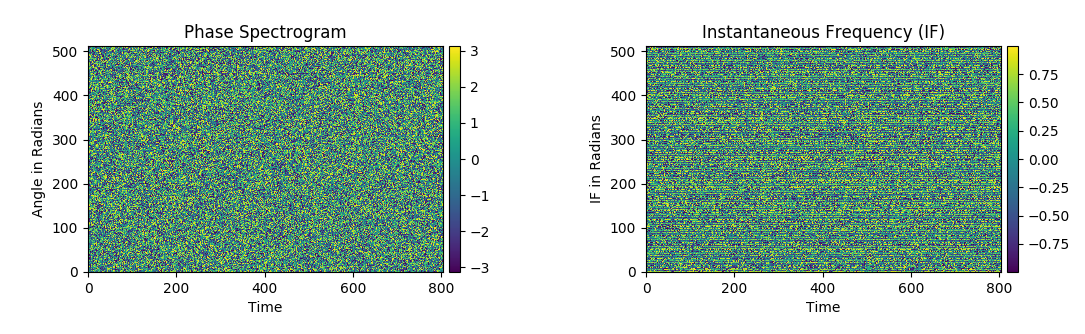
\includegraphics[width=0.85\columnwidth, height=0.40\columnwidth]{master_thesis_template/figs/phase_res.png}
    %\caption{On left is time-phase representation of signal and on right is the instantaneous frequency (IF) representation of a signal illustrated in Figure~\ref{fig:speech_ex}.}
    \caption[Phase and IF representation of a speech signal]{The time-phase representation (left) and the instantaneous frequency (IF) representation (right) of the signal illustrated in Figure~\ref{fig:speech_ex}.}
    \label{fig:phase_response}
\end{figure}

In this work, we present two frameworks of GANs for unsupervised cross-domain speech-to-speech synthesis. In the first framework, we use the magnitude spectrogram of a speech signal and use iterative algorithms for waveform reconstruction. Since the consistency of the spectrogram is a critical requirement to obtain a valid time-domain waveform. We define a spectrogram consistency loss to constrain the generator. In the second framework, we utilize the complete time-frequency representation by combining the magnitude spectrogram and the IF representation of the phase spectrogram. Thus we avoid the use of iterative methods for signal reconstruction and we use the consistency condition of the complete time-frequency representation to define a spectrogram consistency loss term for the generator networks. We discuss the details in Section~\ref{subsec:fsg}.

Our results show the effectiveness of the approach for the cross-domain speech-to-speech synthesis. To evaluate the quality and diversity of generated samples we compute the inception score (IS), the Fr\'{e}chet inception distance (FID) and domain accuracy. The IS and FID require the feature representation of the spectrogram. We train a time-delay neural network (TDNN) model for the speaker identification task and later use it as a feature extractor.
For domain accuracy, we train a binary classifier to discriminate between the voice of male and female speakers. We then compare the accuracy of the classifier on the true set of spectrograms and on the generated set of spectrograms. Furthermore, we also perform the qualitative evaluation of generated speech samples. We performed two perceptual tests to evaluate the quality of speech of generated samples and the extent to which generated samples sounds like a female or a male voice. 

We summarize the main contribution of our work as follows:
\begin{enumerate}[label=(\roman*)]
\item Our network inspired by the UNIT architecture works on the shared latent space assumption. To our knowledge, this setup has not been used previously for speech-to-speech synthesis.

\item We impose the spectrogram consistency constraint on our cross-domain speech-to-speech synthesis network. This allows faster convergence of iterative algorithms and provides a coherent time-domain waveform reconstruction. 

\item We train our framework on the LibriSpeech (\cite{panayotov2015librispeech}) corpus of $251$ speakers and evaluate it on the completely unseen set of $40$ speakers.  

\item We propose to generate the full spectrogram representation where we use the IF representation of the phase along with the magnitude spectrogram. Furthermore, we propose a loss term exploiting consistency of full spectrogram.
\end{enumerate}


Our framework was effective at the task of voice conversion. We achieved quantitative as well as qualitative improvements by imposing the spectrum consistency constraint. In the case of a full time-frequency representation, we observed that the network added artifacts like, echoing in generated speech samples. We attribute this to the different nature of magnitude and phase spectrogram. The magnitude representation is sparse, and phase representation is dense, and combining them as two channels makes it difficult for the network. We think it can be improved by performing extensive hyperparameter tuning, especially hyperparameter of the magnitude and phase term in the loss function as well as of the spectrogram consistency term. Due to limited time and high computational cost of our framework, we left this as future work.

\section{Thesis Outline}
We structure the thesis as follows. In Chapter~\ref{ch:background} we review concepts of signal processing, DL and GMs specifically required for the understanding of our work. In Chapter~\ref{ch:unvc} we formally define the problem statement and discuss the formulation of our framework and training setup. In Chapter~\ref{ch:results}
we explain our evaluation setup, report results along with an extensive discussion of various setups. Finally, we conclude our work in Chapter~\ref{ch:conclusion} along with the discussion on the prospects of this work.




%Thus to smooth out such effect the time-frequency representation are computed using highly overlapping window over a short duration of time intervals. 






%Thus to generate a full spectrum representation is done in two possible ways. requires a right combination of phase and magnitude information


%The application of GM for speech data is limited. In~\cite{oord2016wavenet} proposed an autoregressive model to generate high quality speech signals from time domain representation. However, the approach is limited due to slow inference time. This is mainly attributed to the high sampling rate of speech signals which make it computationally challenging to generate speech signal in real time. Recently, several GAN based approaches~\cite{engel2019gansynth},~\cite{marafiotiadversarial} have been proposed for generating high quality audio data. 



%This is mainly due to the high sampling rate of speech signals which make it computationally challenging to generate time domain signal. Though some generative models like WaveNet work in time domain but they are very slow in inference time and thus are not suitable in real time.

%
